\documentclass[a4 paper]{article}
%\usepackage{minted}           %embedding code
\usepackage{amsmath, amsthm, amsfonts} %always use amsmath for symbols, amsthm for theorems 
\usepackage{graphicx}  % for pictures
%\usepackage{lipsum}  % for test text
\usepackage{multicol}    % for multicollumn text
\usepackage[bottom=2.5cm]{geometry}   %to set the margins to your liking
\usepackage[skip = 10pt, indent = 30pt]{parskip}      %to set the distance between paragraphs
\usepackage{tcolorbox}           %for literal color boxes
%\usepackage{witharrows}             % understandable, arrows for equations
\usepackage{tikz}                   %drawings and diagrams
\usetikzlibrary{positioning}        %tikz library for positioning (of nodes?)
\usepackage{pgfplots}               %plotting and graphs
\pgfplotsset{compat=1.18, width = 10cm}
\usepackage{hyperref}
\hypersetup{colorlinks = true, linkcolor = black, urlcolor = blue}
%\usepackage{fancyvrb}           % fancy formatting of verbatim
%\usepackage{fancyhdr, lastpage}
%\pagestyle{fancy} 
%\lhead{Relat\'orio experimento 4}
%\rhead{FisExpI}
%\cfoot{Página \thepage \ de \pageref{LastPage}}
%\usepackage[Bjornstrup]{fncychap} %Sonny, Glenn, Lenny, Conny, Rejne, Bjarne, Bjornstrup
%\usepackage{xcolor}      %color text
%\usepackage{siunitx}    %for SI units
\usepackage{setspace}
\onehalfspacing
\usepackage{cleveref}
\usepackage[brazil]{babel}
\usepackage{caption}
\usepackage{subcaption}
\usepackage{pdfpages}
\usepackage{booktabs}
\usepackage{multirow}
\usepackage{textcomp}
\usepackage{amssymb}
\usepackage[document]{ragged2e}
\usepackage{bm}
\usepackage{empheq}




%\setlength{\hoffset}{-2cm}
%\setlength{\voffset}{1.5cm}                     %control your margins however you want!
%\setlength{\marginparwidth}{2cm}
%\setlength{\oddsidemargin}{0cm}

%\newtheorem{theorem}{Theorem}[section]               %how you call it and how you display it
%\newtheorem{corollary}{Corollary}[theorem]


\newcommand{\parag}{\hspace{30pt}}
%\newcommand{\pd}[2]{\frac{\partial#1}{\partial#2}}


\begin{document}

\justifying
\begin{center}{\large Laboratório de Circuitos Elétricos - 02/2024 - Turma 05}\\
{\large \textbf{Experimento 9}}\\ 
23/01/2025
\end{center}

\vspace{500pt}
 \noindent\textbf{Grupo 5:}\\
 Yuri Shumyatsky - 231012826\\
Vinicius de Melo Moraes - 231036274\\



\vspace{30pt}
\newpage

\section{Introdução}

\section{Materiais}

	\begin{itemize}
	\item 1 capacitor de 100 nF
	\item 1 resistor de 1k$\Omega$
	\item National Instruments Elvis II (Elvis)
	\end{itemize}

\newpage
\section{Procedimentos}
\parag Primeiro é feita a análise dos componentes usando o multímetro e medidor de impedância do Elvis. Os resultados são dispostos na Tabela 1.

\vspace{5pt}
\begin{table}[h]
\centering
\begin{tabular}{|c|c|c|c|}
\hline
\textbf{Grandeza} & \textbf{Valor nominal} & \textbf{Valor medido} & \textbf{Erro (\%) }\\\hline
R & 47$\Omega$ & 47.359$\Omega$ & 0.76 \\\hline 
L & 1mH & 0.863mH & 13.70 \\\hline 
C & 100nF & 107.500nF & 7.50 \\\hline 
\end{tabular}
\caption*{Tabela 1: Valores dos componentes}
\end{table}

Em seguida, esses componentes são usados para montar o circuito exposto na Figura 1.

\begin{table}[h]
\centering
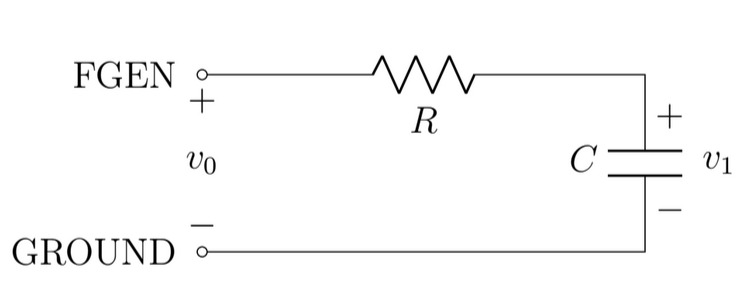
\includegraphics[scale=0.4]{figuras/figura1}
\end{table}
\begin{center}
Figura 1: Disposição do Circuito 1
\end{center}

O gerador de funções do Elvis é configurado para gerar uma onda triangular com 2$V_{pp}$, offset zero e frequência de 1kHz. Assim, é gerada a onda do Gráfico 1.

\begin{table}[h]
\centering
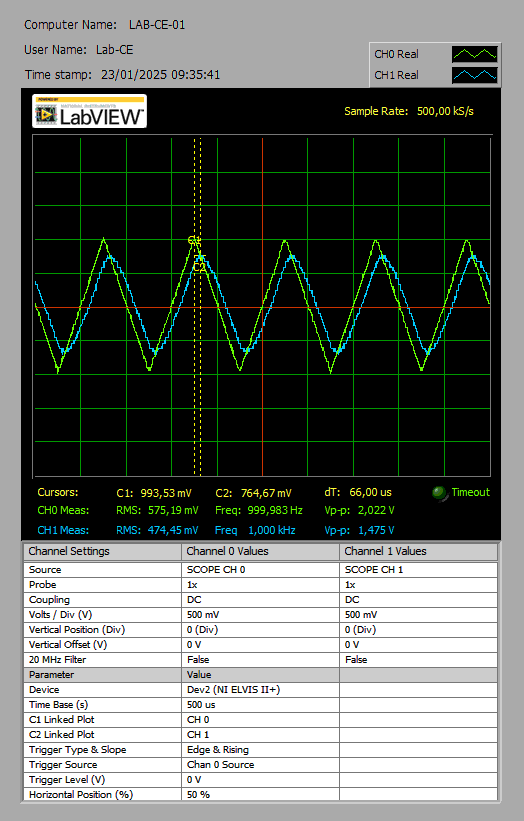
\includegraphics[scale=0.8]{graficos/rgadicoa1-triangulo}
\end{table}
\begin{center}
Gráfico 1: Onda Triangular
\end{center}

%grafico do teorico

%calculo da serie de fourier da triangular
Agora, sabendo que 

\begin{equation*}
v_0(t)=\left\{
\begin{array}{lr}
1+4f_0t,\hspace{10pt} -\frac{T}{2}<t\leq0\\
1-4f_0t,\hspace{10pt} 0<t\leq\frac{T}{2}
\end{array}\right.
\end{equation*}

com $f_0=1kHz$ e que a sua série de Fourier é

\begin{equation*}
v_0(t)=
\begin{array}{lr}
\sum\limits_{m=1}^\infty A_m cos (2\pi(2m-1)f_0t)
\end{array}
\end{equation*}

%calculo Am

Em seguida, vamos calcular a resposta do sistema para os harmônicos de frequências 1, 3, 5, 7, 9, 11, 13, 15, 17 e 19 kHz.

%calculo

Agora experimentalmente são medidas as mesmas respostas, que seguem nos Gráficos 2 a 11. 

\newpage\begin{table}[h]
\centering
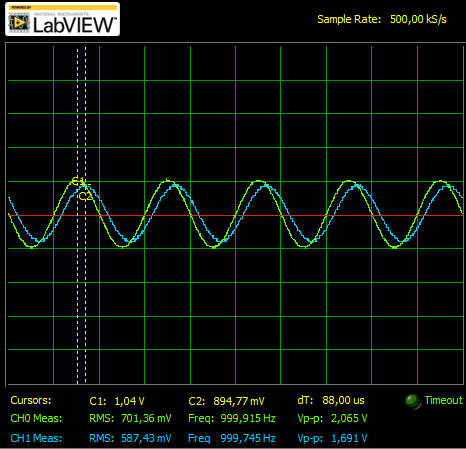
\includegraphics[scale=0.7]{graficos/RGADICOA1}
\end{table}
\begin{center}
Gráfico 2: Resposta para Frequência 1kHz
\end{center}


\begin{table}[h]
\centering
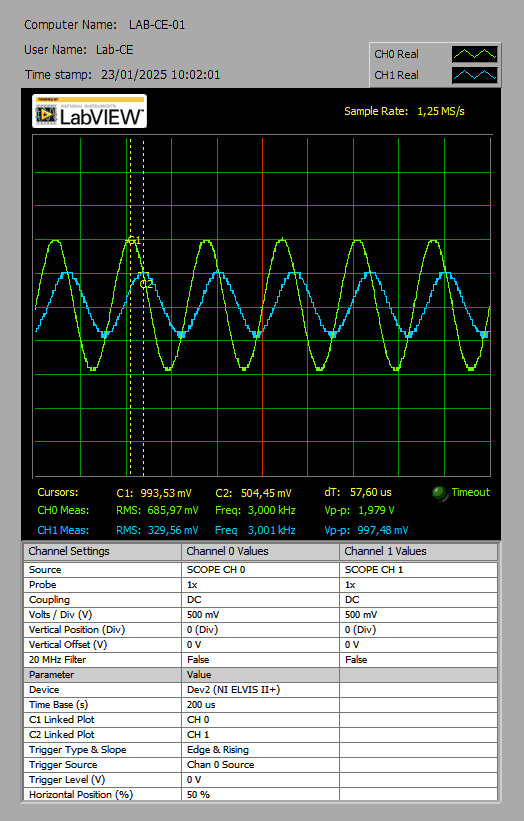
\includegraphics[scale=0.7]{graficos/RGADICOA3}
\end{table}
\begin{center}
Gráfico 3: Resposta para Frequência 3kHz
\end{center}

\newpage
\begin{table}[h]
\centering
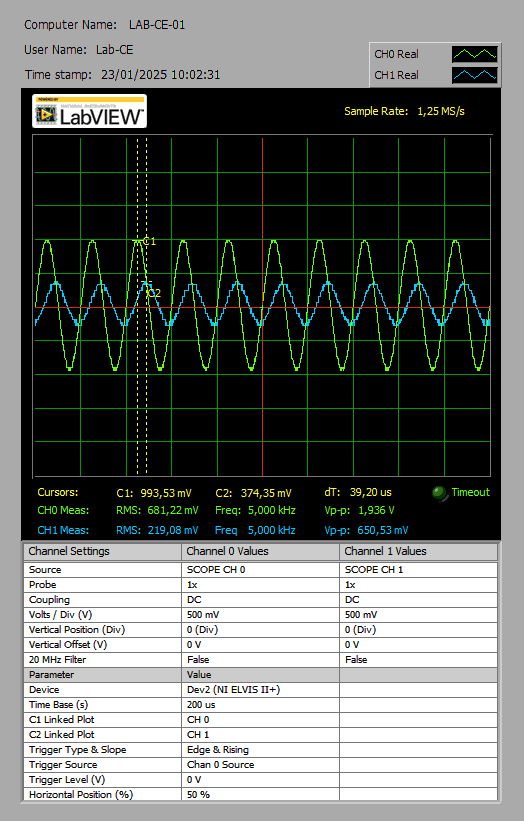
\includegraphics[scale=0.7]{graficos/RGADICOA5}
\end{table}
\begin{center}
Gráfico 4: Resposta para Frequência 5kHz
\end{center}


\begin{table}[h]
\centering
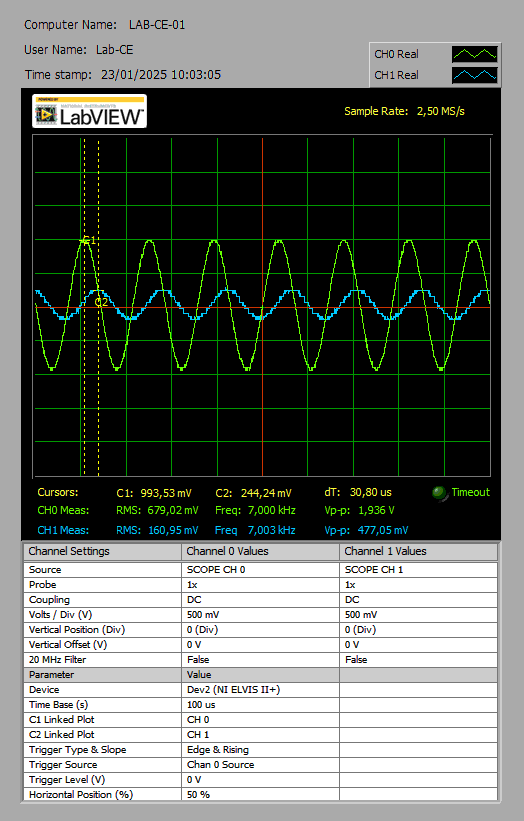
\includegraphics[scale=0.7]{graficos/RGADICOA7}
\end{table}
\begin{center}
Gráfico 5: Resposta para Frequência 7kHz
\end{center}

\newpage
\begin{table}[h]
\centering
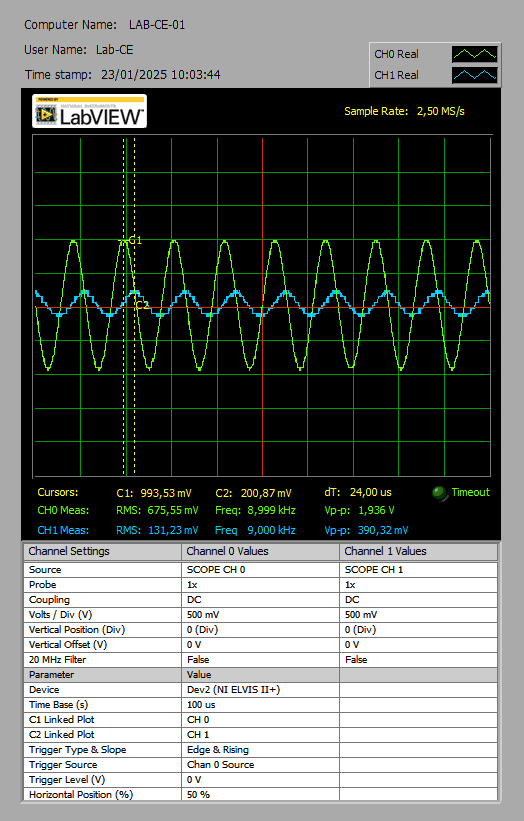
\includegraphics[scale=0.7]{graficos/RGADICOA9}
\end{table}
\begin{center}
Gráfico 6: Resposta para Frequência 9kHz
\end{center}


\begin{table}[h]
\centering
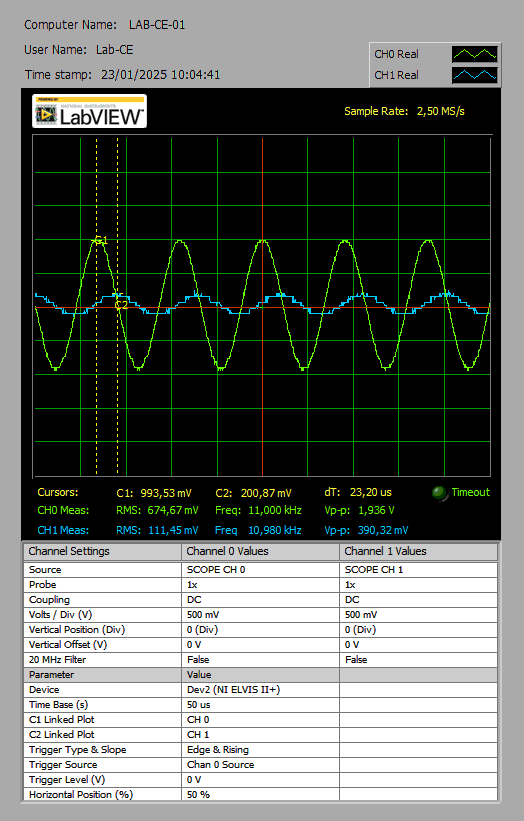
\includegraphics[scale=0.7]{graficos/RGADICOA11}
\end{table}
\begin{center}
Gráfico 7: Resposta para Frequência 11kHz
\end{center}

\newpage
\begin{table}[h]
\centering
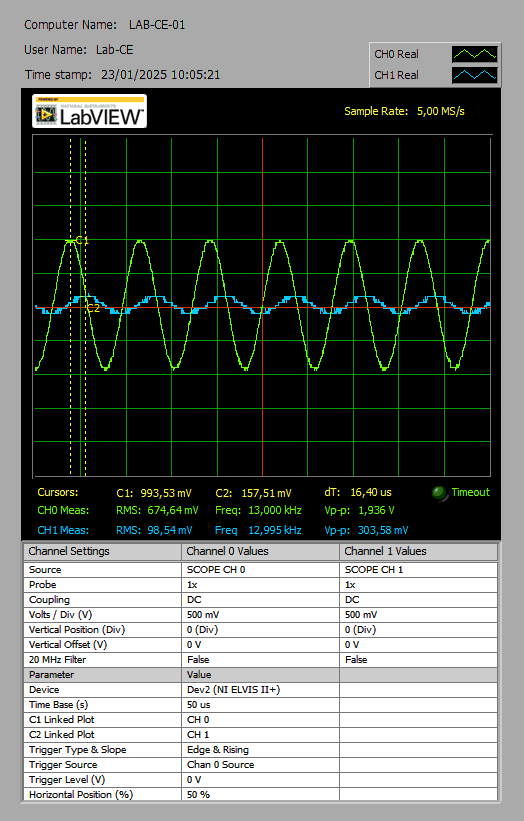
\includegraphics[scale=0.7]{graficos/RGADICOA13}
\end{table}
\begin{center}
Gráfico 8: Resposta para Frequência 13kHz
\end{center}


\begin{table}[h]
\centering
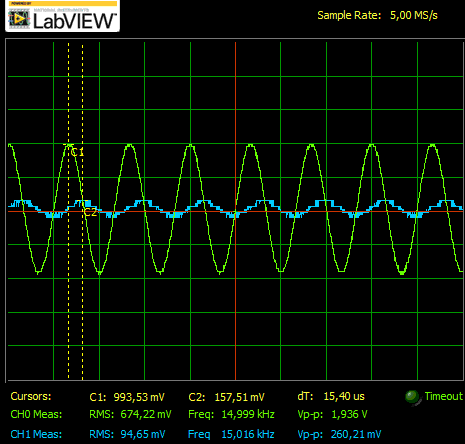
\includegraphics[scale=0.7]{graficos/RGADICOA15}
\end{table}
\begin{center}
Gráfico 9: Resposta para Frequência 15kHz
\end{center}

\newpage
\begin{table}[h]
\centering
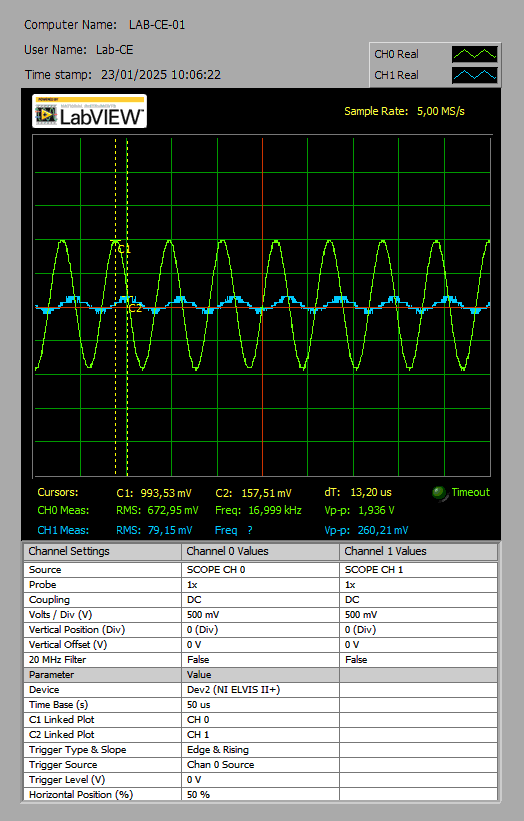
\includegraphics[scale=0.7]{graficos/RGADICOA17}
\end{table}
\begin{center}
Gráfico 10: Resposta para Frequência 17kHz
\end{center}


\begin{table}[h]
\centering
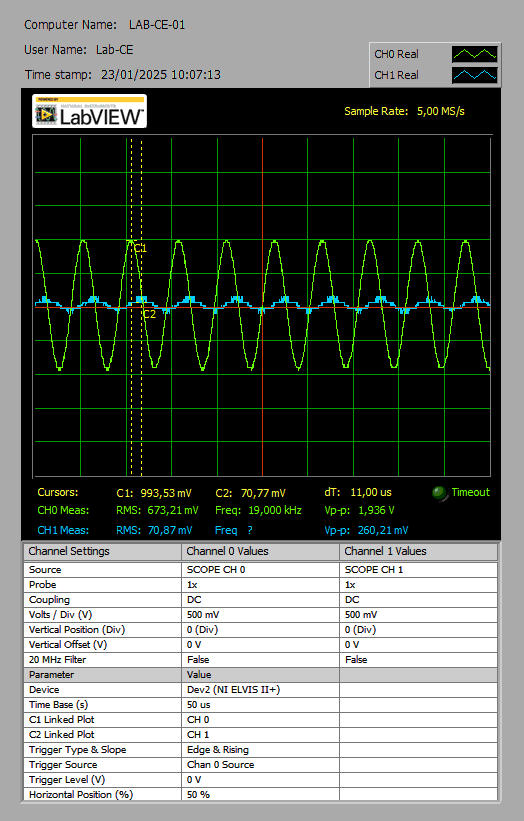
\includegraphics[scale=0.7]{graficos/RGADICOA19}
\end{table}
\begin{center}
Gráfico 11: Resposta para Frequência 19kHz
\end{center}

Desses gráficos são extraídas as informações da Tabela 2.
\newpage

\vspace{5pt}
\begin{table}[h]
\centering
\begin{tabular}{|c|c|c|c|c|}
\hline
\textbf{Frequência (kHz)} & \textbf{Grandeza} & \textbf{Valor nominal} & \textbf{Valor medido} & \textbf{Erro (\%) }\\\hline
10   & $|V_0|$ & 1.57V & 1.55V & 1.27 \\\hline
10   & $|V_1|$ & 2.33V & 1.81V & 22.31 \\\hline
10   & $20log_{10}(|V_1|/|V_0|)$ & 3.434 & 1.347 & 60.77 \\\hline
10   & Fase de $V_1$ em relação a $V_0$ & -26.01\textdegree & -43.20\textdegree & 66.09 \\\hline
12.5 & $|V_0|$ & 1.25V & 1.38V & 10.40 \\\hline
12.5 & $|V_1|$ & 2.35V & 1.63V & 30.64 \\\hline
12.5 & $20log_{10}(|V_1|/|V_0|)$ & 5.481 & 1.446 & 73.62 \\\hline
12.5 & Fase de $V_1$ em relação a $V_0$ & -43.93\textdegree & -57.24\textdegree & 30.30 \\\hline
15.5 & $|V_0|$ & 0.97V & 1.34V & 38.14 \\\hline
15.5 & $|V_1|$ & 2.11V & 1.46V & 30.81 \\\hline
15.5 & $20log_{10}(|V_1|/|V_0|)$ & 6.733 & 0.745 & 88.94 \\\hline
15.5 & Fase de $V_1$ em relação a $V_0$ & -83.58\textdegree & -71.45\textdegree & 14.51 \\\hline
19.3 & $|V_0|$ & 1.17V & 1.34V & 14.53 \\\hline
19.3 & $|V_1|$ & 1.58V & 1.20V & 24.05 \\\hline
19.3 & $20log_{10}(|V_1|/|V_0|)$ & 2.626 & -0.958 & 136.48 \\\hline
19.3 & Fase de $V_1$ em relação a $V_0$ & -129.54\textdegree & -94.48\textdegree & 27.06 \\\hline
24.1 & $|V_0|$ & 1.51V & 1.47V & 2.65 \\\hline
24.1 & $|V_1|$ & 1.02V & 0.89V & 12.75 \\\hline
24.1 & $20log_{10}(|V_1|/|V_0|)$ & -3.381 & -4.359 & 28.93 \\\hline
24.1 & Fase de $V_1$ em relação a $V_0$ & -151.17\textdegree & -121.47\textdegree & 19.65 \\\hline
30   & $|V_0|$ & 1.72V & 1.64V & 4.65 \\\hline
30   & $|V_1|$ & 0.64V & 0.63V & 1.56 \\\hline
30   & $20log_{10}(|V_1|/|V_0|)$ & -8.635 & -4.155 & 51.88 \\\hline
30   & Fase de $V_1$ em relação a $V_0$ & -160.86\textdegree & -129.49\textdegree & 19.51 \\\hline
\end{tabular}
\caption*{Tabela 2: Valores referentes ao circuito 1}
\end{table}

Agora, com esses valores e o $A_m$, será calculado $\hat{v_1}(t)$ com os valores teóricos e medidos, considerando que 

\[\hat{v_1}(t)=\sum\limits_{m=1}^{10}A_m|V_1((2m-1)f_0|cos(2\pi(2m-1)f_0t+\phi(V_1((2m-1)f_0)))\]

com $f_0=1kHz, |V_1(f)|$ a amplitude de $v_1$ na frequência $f$ e $phi(V_1(f))$ a fase de $v_1$ em relação a $v_0$ nesse mesmo caso.



\section{Conclusão}

\section{Bibliografia}

\begin{itemize}
\item HALLIDAY, D.; RESNICK, R.; WALKER, J. Fundamentos de Física. 10. ed. v. 3. Rio de Janeiro: LTC, 2016.
\end{itemize}

\end{document}